\section{Architetture}\label{capitolo2}
I sistemi distribuiti sono spesso definibili come pezzi di software sparsi su molte macchine. Al fine di dominare la loro complessità è necessario che questi sistemi siano organizzati. Un modo semplice per distinguere l'organizzazione di un sistema distribuito, è quello di distinguere l'organizzazione logica dei componenti software e la relativa realizzazione fisica.\\
Per \emph{architetture software} intendiamo l'organizzazione e l'interazione dei vari componenti software; mentre l'effettiva realizzazione di un sistema distribuito richiede che i componenti software siano istanziati su macchine reali, l'architettura risultante viene detta \emph{architettura di sistema}.Analizzeremo per prime le architetture centralizzate in cui un server implementa la maggior parte delle funzionimentre client remoti accedono al server tramite semplici mezzi di comunicazione.\\
\subsection{Stili architetturali}
Iniziamo l'analisi dalle diverse tipologie di architetture software in quanto progettazione e adozione di una adeguata architettura sono fondamentali per la riuscita e la manuntenibilità del sistema.\\
Introduciamo ora la nozione di \emph{stile architetturale} che esprime in termini di componenti mezzi di comunicazione e messaggi scambiati. Un \emph{componente} è un'unità modulare con interfacce ben definite e sostituibile nel suo ambiente.\\
La comunicazione tra i diversi componenti avviene tramite quello che è definito \emph{connettore} ovvero un sistema che implementa le chiamate a procedure remote piuttosto che il passaggio di messaggi o lo streaming dei dati.\\
Usando componenti e connettori possiamo ottenere diverse configurazioni che a loro volta sono classificati in diversi \emph{stili architetturali}. I più importanti stili architetturali ad oggi identificati sono:
\begin{itemize}
\item architettura a livelli (\emph{layer})
\item architetture basate sugli oggetti
\item architetture centrate sui dati
\item architetture basate sugli eventi
\end{itemize}
Per quanto riguarda lo stile a livelli è quello più semplice nel quale i componenti sono organizzati a strati in cui un componente del livello $L_i$ può chiamare un componente del livello $L_{i-1}$ ma non può contattare i componenti dello stesso livello. Questo modello è uno dei più utilizzati nelle applicazioni di rete, le richieste scendono lungo la catena gerarchica mentre le risposte risalgono.\\
Le \emph{architetture basate sugli oggetti} hanno un organizzazione meno rigida, ogni oggetto corrisponde ad un componente e tutti gli oggetti sono connessi tramite \emph{chiamate a procedura remota}; questo tipo di architettura corrisponde esattamente al caso client-server ed insieme a quella a livelli costituiscono il 90\% delle architetture dei sistemi distribuiti presenti oggi.\\
Le \emph{architetture basate sui dati} si sviluppano attorno all'idea che i processi comunicano attraverso un \emph{repository} comune.\\
Nelle \emph{architetture basate sugli eventi} i processi comunicano essenzialmente attraverso la propagazione degli eventi, i più noti tipi di sistemi distribuiti che utilizzano la propagazione degli eventi sono i sistemi \emph{publish/subscribe} nei quali alcuni processi pubblicano degli eventi ed è il middleware ad assicurarsi che questi eventi siano ricevuti soltanto da qui processi che si sono iscritti a quel determinato evento.\\
Nel caso in cui si combinino le architetture basate sugli eventi con quelle basate sui dati si ottiene una architettura chiamata \emph{spazio di dati condivisi} che permette ai processi di essere disaccoppiati anche nel tempo in quanto non è necessario che i processi siano attivi nell'istante in cui avviene la comunicazione.
\subsection{Architetture di sistema}
Abbiamo visto fino ad ora alcune scelte architetturali, vediamo ora come sono effettivamente organizzati la maggior parte dei sistemi distribuiti considerando dove sono posizionati i componenti software. La scelta di quali componenti usare e di come posizionarli porta alla realizzazione della cosiddetta \emph{architettura di sistema}.
\subsection{Architetture centralizzate}
La prima architettura che analizzeremo è quella \emph{centralizzata}, in quanto pensare ad un sistema in termini di \emph{client} che richiedono dei servizi a dei \emph{server} facilita la comprensione e la gestione dei sistemi distribuiti.\\
Nel modello client-server i processi sono suddivisi in due gruppi; un \textbf{server} è un processo che implementa uno specifico servizio. Un \textbf{client} è invece un processo che richiede un servizio ad un serve inviandogli una richiesta e quindi attendendo una risposta.\\
La comunicazione tra client e server può essere implementata per mezzo di un semplice protocollo senza connessione quando la rete sottostante è molto affidabile. In questo caso quando un client richiede un servizio invia un messaggio al server indicando il servizio richiesto e i dati di input. Quest'ultimo all'arrivo della richiesta la processa e confeziona i risultati in un altro messaggio.\\
L'utilizzo di un protocollo senza connessione ha il vantaggio di essere efficiente fino a quando non abbiamo perdita di pacchetti. Si potrebbe pensare di impostare il client affinché rinvii il messaggio quando non riceve alcuna rsposta, ma non si può stabilire se è stato perso il messaggio o la risposta e quindi il server ha compiuto oppure no l'operazione richiesta. In alcuni casi le richieste sono \emph{idempotenti} ovvero possono essere ripetute senza danni.\\
Per risolvere il problema della perdita di messaggi, molte architetture client-server utilizzano dei protocolli affidabili orientati alla connessione.
\paragraph{Stratifficazioni delle applicazioni}
Il problema principale dell'architettura client server è che non vi è una netta distinzione tra quali sono le funzionalità del client e quelle del server; è stata così introdotta una un nuovo tipo di suddivisione delle diverse funzionalità in base che esse siano più vicine all'utente o ai dati. I tre livelli identificati sono:
\begin{itemize}
\item il livello dell'interfaccia utente
\item il livello applicativo
\item il livello dei dati
\end{itemize}
Il livello dell'interfaccia utente contiene tutto ciò che è necessario per interfacciarsi con l'utente come la gestione della grafica. Il livello applicativo di solito contiene le applicazioni. Il livello dei dati gestisce tutto ciò che concerne i dati da gestire.\\
Esistono diversi modi in cui questi tre livelli possono essere istanziati sull'hardware come possiamo vedere in \figurename~\ref{fig:layer}.
La configurazione più utilizzata è quella nel quale il client implementa solo il livello dell'interfaccia utente (\emph{thin client}) ma esistono altri sistemi una parte dal livello applicativo si trova implementata nel client, in questo caso si parla di \emph{fat client}.
\begin{figure}[htb]
\centering
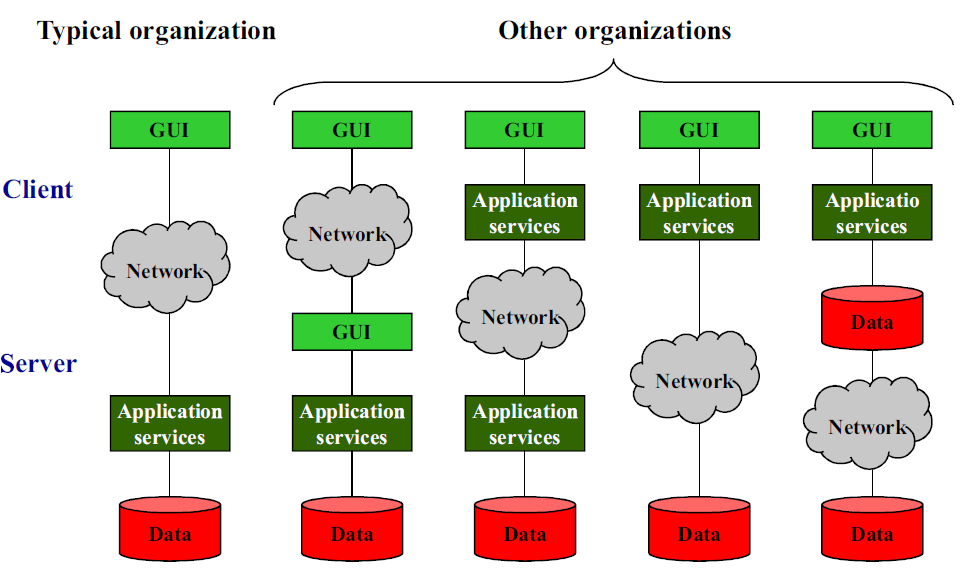
\includegraphics[width=8cm]{img/layer.png}\\
\caption{Esempio di suddivisione dei layer}\label{fig:layer}
\end{figure}
Per quanto riguarda il livello dei dati molte volte è gestito da meccanismi che rendono i dati \textbf{persistenti} anche quando non vi sono altre applicazioni in esecuzione. In alcuni casi molto semplici il livello dei dati consiste in un  \emph{filesystem} ma nella maggioranza dei casi si tratta di una \emph{base di dati}
\paragraph{Architetture multi livello}
La suddivisione delle applicazioni in tre livelli logici suggerisce anche una distribuzione fisica delle applicazioni client serversu molte macchine, la distribuzione più semplice è quella su due macchine:
\begin{enumerate}
\item una macchina client che contiene solo i programmi dell'interfaccia utente
\item una macchina server contenete il resto dei programmi e i dati
\end{enumerate}
Si possono suddividere le applicazioni anche in altri modi come visto in \figurename~\ref{fig:layer}.\\
La tendenza degli ultimi anni è quella di suddividere i diversi livelli su più macchine in modo da creare una architetture multi livello.
Un esempio pratico ad esempio è quello mostrato in \figurename~\ref{fig:3layer} nella quale si mostra un architettura a 3 livelli.\\
\begin{figure}[htb]
\centering
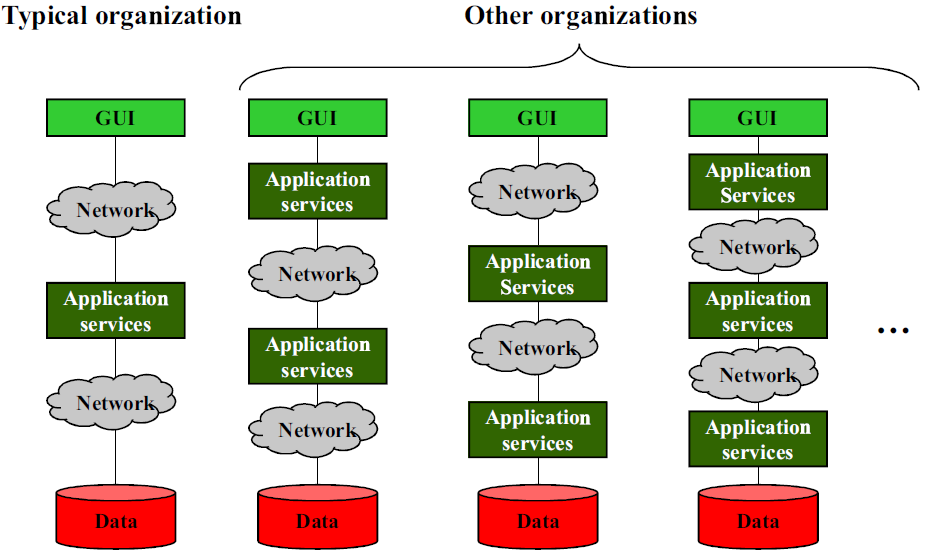
\includegraphics[width=8cm]{img/3layer.png}
\caption{Esempio di suddivisione dei layer su 3 livelli}\label{fig:3layer}
\end{figure}
\subsubsection{Architetture decentralizzate}
La suddivisione delle architetture client server in livelli denota un tipo di distrinuzione detta \emph{verticale} in quanto i componenti sono divisi su più macchine seguendo un criterio \emph{logico}.\\
Questo tipo di distribuzione è utile con le architetture client-server ma nel caso in cui la distribuzione che conta è quella dei client e dei server e non delle funzioni allora si parla di \emph{frammentazione orizzontale}. Un esempio molto conosciuto di architettura con distribuzione orizzontale sono i \textbf{sistemi peer-to-peer}.\\
I processi che costituiscono un sistema peer-to-peer sono tutti uguali, di conseguenza l'interazione tra processi è quasi del tutto simmetrica e i processi agiscono sia da client che da server e per questo sono anche detti \textbf{servent}.\\
Dato questo tipo di comportamento il problema principale delle reti \emph{p2p} è quello di organizzare i processi in una rete \emph{overlay} ovvero una rete nella quale i processi costituiscono i nodi e i collegamenti rappresentano i canali di comunicazione. Con questa struttura un processo non può comunicare direttamente con un altro processo arbitrario ma deve seguire i canali di comunicazione disponibili.\\
Esistono due tipi principali di reti \emph{overlay} quelle strutturate e quelle non strutturate.
\paragraph{Architetture peer-to-peer strutturate}
In una rete p2p strutturata la rete overlay è costruita usando una procedura deterministica, quella più comune è l'uso di una \textbf{hash tabel distribuita} (DHT). In questo tipo di struttura ai dati viene assegnato un identificatore univoco in uno spazio molto grande (129:160 bit). Anche ai nodi del sistema viene assegnato un identificatore nello stesso spazio dei dati. Il punto cruciale di questa architettura è quello di creare uno schema efficiente e deterministico che associ univocamente la chiave di un dato con l'identificativo di un nodo basandosi su un'opportuna metrica di distanza. Inoltre, è importante che quando si effettua la ricerca di un dato sia restituito l'indirizzo del nodo al quale questo dato è associato, e ciò si ottiene \emph{instradando} la richiesta al nodo associato.\\
Ad esempio nel sistema \emph{Chord} i nodi sono organizzati logicamente ad anello, ed i dati sono organizzati assegnando i dati con identificativo $k$ al nodo con più piccolo identificativo $id>k$; questo nodo è chiamato \emph{successore} della chiave $k$ ed è identificato come $succ(k)$ come mostrato in \figurename~\ref{fig:chordring}.\\
\begin{figure}[htb]
\centering
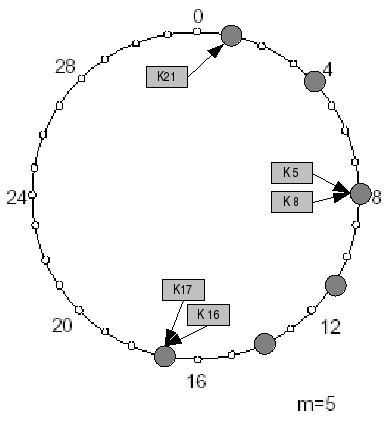
\includegraphics[width=8cm]{img/chordring.jpg}\\
\caption{Esempio di sistema Chord}\label{fig:chordring}
\end{figure}
La parte più importante della gestione di una rete overlay strutturata è la \textbf{gestione dell'appartenenza} da parte dei nodi. Quando un nodo vuole unirsi alla rete genera un \emph{id} casuale ed effettua una ricerca di $id$ a questo punto il sistema restituirà $succ(id)$. Alla fine per inserirsi il nuovo nodo contatterà il successore individuato dalla ricerca e il suo predecessore e si inserirà nell'anello. Inoltre, l'inserimento causa la migrazione dei dati associati ad $id$ da $succ(id)$.
L'uscita è molto semplice il nodo informa della sua dipartita il $succ(id)$ e il suo predecessore e trasferisce i dati a $succ(id)$.\\
\paragraph{Architetture peer-to-peer non strutturate}
I sistemi peer-to-peer non strutturati si basano su algoritmi casuali per costruire la rete \emph{overlay}. L'idea è quella che ogni nodo mantenga una lista dei suoi vicini. Inoltre, anche i dati sono posizionati sui nodi in modo casuale, di conseguenza l'unico modo di effettuare una ricerca è inoltrare la richiesta a tutta la rete.\\
L'obiettivo principale di un sistema p2p non strutturato è la creazione di un \textbf{grafo disordinato}. Per fare ciò ogni nodo mantiene una lista di $c$ vicini scelti a caso dall'insieme dei nodi \emph{vivi}; questa vista è detta \textbf{vista parziale}.
Ora supponiamo che un nodo voglia aggiungersi alla rete, esso contatta in altro nodo arbitrario dalla lista dei punti di accesso; questo punto di accesso è un normale nodo della rete che però ha un alta probabilità di essere disponibile. I meccanismi che creano la rete overlay sono detti \emph{push} e \emph{pull} e permettono lo scambio delle informazioni per la costruzione della rete tra i nodi. Questi meccanismi usati singolarmente possono portare alla creazione di reti overlay disconnesse, per questo si usano entrambe le tecniche.\\
L'uscita dalla rete è molto semplice, infatti, visto che i nodi si scambiano periodicamente le viste parziali basta solo che il nodo lasci la rete, gli altri nodi con il passare del tempo si accorgono dell'assenza del nodo che ha lasciato la rete e lo elimina dalla sua vista parziale.
\paragraph{Gestione della topologia di una rete overlay}
Anche se i sistemi p2p strutturati e non strutturati sembrano costruire due classi completamente diverse, in realtà selezionando attentamente gli elementi scambiati nelle viste parziali è possibile costruire reti overlay con tipologie specifiche. Un esempio molto interessante sono quelle funzioni che cercano di cogliere la \textbf{vicinanza semantica} dei dati che creano reti \textbf{overlay semantiche} che permettono ricerche efficienti nei sistemi p2p non strutturati.
\paragraph{Superpeer}
Specialmente nelle reti non strutturate al crescere delle dimentsioni potrebbe diventare problematico localizzare i dati. Questo è dovuto al fatto non esiste un modo deterministico per instradare una richiesta di ricerca.\\
Per evitare questo problema molte reti p2p hanno proposto l'utilizzo di nodi speciali che mantengono un indice dei dati. Questo tipo di nodi sono detti \textbf{superpeer}. I superpeer sono organizzati tra loro tramite una rete p2p; si forma così una struttura ad albero. L'accesso ad un normale peer avviene attraverso l'accesso al superpeer.
\subsubsection{Architetture ibride}
Fino ad ora abbiamo visto le architetture centralizzate client-server e alcune architetture peer-to-peer ora vediamo come queste due tipologie di architetture possono combinarsi per dare vita ad altre architetture dette \emph{ibride}
\paragraph{Sistemi edge-server}
I sistemi \emph{edge-server} sono una classe molto diffusa di architetture ibride. In questa classe i server sono posti ai bordi della rete Internet ovvero tra la rete Internet e quelle aziendali come nel caso degli \textbf{Internet service provider}. I client si connettono alla rete internet tramite un edge-server il quale fornisce i contenuti dopo aver applicato dei filtri e funzioni di transcodifica.
\paragraph{Sistemi distribuiti collaborativi}
Le strutture ibride sono largamente utilizzate nei sistemi distribuiti collaborativi dove sono necessarie velocità nell'entrare nel sistema e per questo viene utilizzato uno schema di tipo client-server. Dopo di che si usa uno schema completamente decentralizzato.\\
Un sistema concreto che utilizza questo meccanismo è il sistema \emph{BitTorrent}
\subsection{Architetture e middleware a confronto}
Considerando le questioni architetturali viste fino ad ora ci chiediamo quale ruolo giochi il middleware visto nei capitoli precedenti.\\
Il middleware in realtà costituisce uno strato tra le applicazioni e le piattaforme distribuite ed il suo obiettivo è quello di fornire un certo grado di trasparenza alla distribuzione. Ciò che accade in realtà è che i middleware seguono uno specifico stile architetturale (ad oggetti come \emph{CORBA} o ad eventi come \emph{TIB/Rendezvous}). Avere un middleware basato su di un certo stile architetturale rende più semplice la progettazione e la realizzazione delle applicazioni.\\
Lo svantaggio più grande è però il fatto che un middleware può  non essere ottimale per una determinata applicazione ciò porta ad avere o middleware molto grandi o a diverse versioni per una specifica classe di applicazioni.
\subsubsection{Interceptor}
Concettualmente un \emph{interceptor} non è altro che un costrutto software che interrompe il normale flusso di controllo e consente ad altro codice di essere eseguito. Rendere però un interceptor generico è molto arduo e a volte averne uno con funzionalità limitate migliorerà sia la gestione del software che che il sistema distribuito nel suo complesso.\\
Il concetto è che un oggetto $A$ può richiamare un metodo appartenete all'oggetto $B$ ache se quest'ultimo risiede su una macchina diversa da $A$.
I passi per eseguire questa chiamata remota sono:
\begin{enumerate}
\item All'oggetto $A$ viene fornita un interfaccia locale esattamente uguale a quella fornita dall'oggetto $B$; a questo punto $A$ richiama il metodo disponibile nell'interfaccia
\item La chiamata di $A$ è trasformata in un'invocazione a un oggetto generico disponibile tramite un'interfaccia generale messa a disposizione dal middleware.
\item L'invocazione a questo oggetto generico viene trasformata in un messaggio inviato attraverso l'interfaccia di rete.
\end{enumerate}
